\documentclass[handout]{beamer}

\usetheme[progressbar=frametitle]{metropolis}
\usepackage{appendixnumberbeamer}
\usepackage{booktabs}
\usepackage{amsmath}
\usepackage{amssymb}
\usepackage{tcolorbox}
\usepackage{tikz}

\definecolor{metropolisblue}{RGB}{39, 59, 94}



% Begin document
\begin{document}

% Title page
\title{Monte Carlo Methods}
\subtitle{Univariate}
\author{Nipun Batra}
\date{\today}
\institute{IIT Gandhinagar}
\maketitle

% Section 1
\section{Introduction}

\begin{frame}{General Form}
The general form of Monte Carlo methods is:
The expectation of a function $f(x)$ with respect to a distribution $p(x)$ is given by:
\begin{equation}
    % Expectation of f(x) with respect to p(x)
    \mathbb{E}_{x \sim p(x)}[f(x)] = \int f(x) p(x) dx
\end{equation}

Using Monte Carlo methods, we can estimate the above expectation by sampling $x_i$ from $p(x)$ and computing the average of $f(x_i)$.
\begin{equation}
    % Monte Carlo estimate of expectation of f(x) with respect to p(x)
    \mathbb{E}_{x \sim p(x)}[f(x)] \approx \frac{1}{N} \sum_{i=1}^{N} f(x_i)
\end{equation}
where $x_i \sim p(x)$.
\end{frame}
\begin{frame}[fragile]{Estimating Pi using Monte Carlo (Part 1)}
    We can estimate the value of pi using Monte Carlo methods by considering a unit square with a quarter circle inscribed within it.
    
    \begin{itemize}
        \item Let $p(x)$ be defined over the unit square using the uniform distribution in two dimensions, i.e., $p(x) = U(x) = 1$ for $x \in [0, 1]^2$.
        \item Let $f(x)$ be the indicator function defined as follows:
            \[
            f(x) = \begin{cases}
                        \text{\textcolor{green}{Green}} (1), & \text{if } x \text{ falls inside the quarter circle}, \\
                        \text{\textcolor{red}{Red}} (0), & \text{otherwise}.
                   \end{cases}
            \]
    \end{itemize}
\end{frame}
    
\begin{frame}[fragile]{Estimating Pi using Monte Carlo (Part 1)}

    \begin{itemize}
    \item Or, we can write $f(x)$ to be the following:
        \[
        f(x) = \begin{cases}
                    1, & \text{if } x_1^2 + x_2^2 \leq 1, \\
                    0, & \text{otherwise}.
               \end{cases}
        \]
    \item Or, using the indicator function, we can write $f(x)$ to be the following:
        \[
        f(x) = \mathbb{I}(x_1^2 + x_2^2 \leq 1)
        \]
    \end{itemize}
    
    \begin{center}
    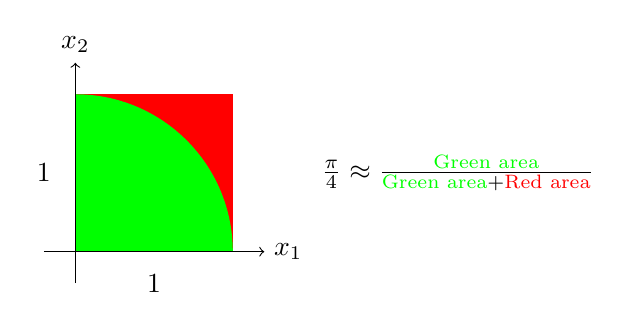
\begin{tikzpicture}[scale=2]
        % Unit Square
        \fill[red] (0,0) rectangle (1,1);
        
        % Quarter Circle
        \fill[green] (0,0) -- (0,1) arc (90:0:1) -- cycle;
        
        % Coordinate Axes
        \draw[->] (-0.2,0) -- (1.2,0) node[right] {$x_1$};
        \draw[->] (0,-0.2) -- (0,1.2) node[above] {$x_2$};
        
        % Labels
        \node at (0.5, -0.2) {1};
        \node at (-0.2, 0.5) {1};
        \node[right] at (1.5, 0.5) {$\frac{\pi}{4} \approx \frac{\text{\textcolor{green}{Green area}}}{\text{\textcolor{green}{Green area}} + \text{\textcolor{red}{Red area}}}$};

    \end{tikzpicture}
    \end{center}
    \end{frame}

    \begin{frame}{Estimaing prior predictive distribution}
        \begin{itemize}
            \item Let $p(\theta)$ be the prior distribution of parameter $\theta \in R^2$. Say, for example, $p(\theta_i) = \mathcal{N}(0, 1) \forall i$.
            \item Let $p(y |\theta, x)$ be the likelihood function. Say, for example, $p(y|\theta, x) = \mathcal{N}(\theta_0 + \theta_1 x, 1)$.
            \item Then, the prior predictive distribution is given by:
        \end{itemize}

            \begin{equation}
                p(y|x) = \int p(y|\theta, x) p(\theta) d\theta 
            \end{equation}

            \begin{equation}
                p(y|x) \approx \frac{1}{N} \sum_{i=1}^{N} p(y|\theta_i, x)
            \end{equation}
            where $\theta_i \sim p(\theta)$.
    \end{frame}

    \begin{frame}{Rejection Sampling}
        \begin{itemize}
            \item Let $p(x)$ be the target distribution from which we want to sample.
            \item Let $q(x)$ be a proposal distribution from which we can sample.
            \item Let $M$ be a constant such that $M \geq \frac{p(x)}{q(x)} \forall x$.
            \item Then, we can sample from $p(x)$ by sampling from $q(x)$ and accepting the sample with probability $\frac{p(x)}{M q(x)}$.
        \end{itemize}
        
    \end{frame}

   \begin{frame}{Rejection Sampling}
    \begin{figure}
        \centering
        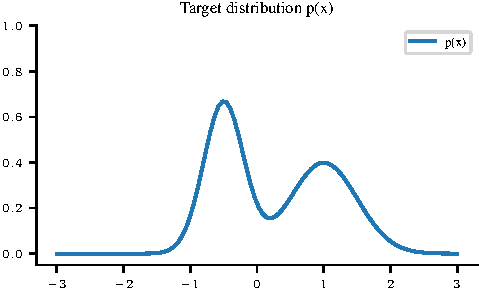
\includegraphics{notebooks/figures/sampling/rejection-sampling--1.0-False-False-False-False-False-False-False-False.pdf}
    \end{figure}
    
   \end{frame}

    \begin{frame}{Rejection Sampling}
        \begin{figure}
            \centering
            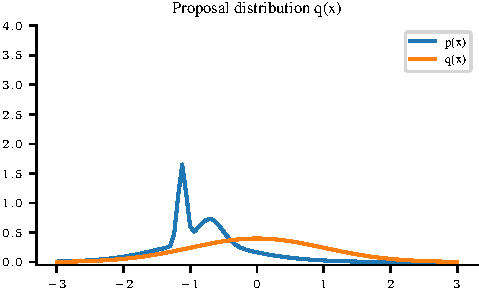
\includegraphics{notebooks/figures/sampling/rejection-sampling--1.0-True-False-False-False-False-False-False-False.pdf}
        \end{figure}
    \end{frame}

    \begin{frame}{Rejection Sampling}
        \begin{figure}
            \centering
            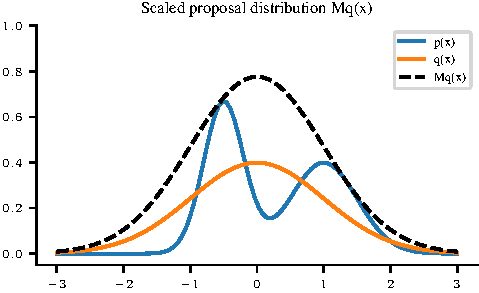
\includegraphics{notebooks/figures/sampling/rejection-sampling--1.0-True-True-False-False-False-False-False-False.pdf}
        \end{figure}
    \end{frame}

    \begin{frame}{Rejection Sampling}
        \begin{figure}
            \centering
            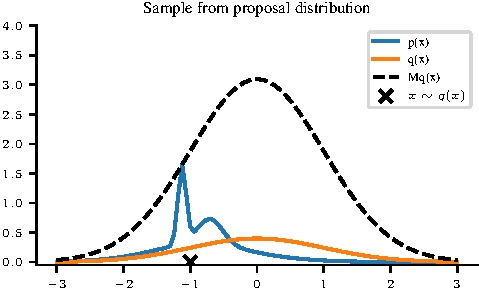
\includegraphics{notebooks/figures/sampling/rejection-sampling--1.0-True-True-True-False-False-False-False-False.pdf}
        \end{figure}
    \end{frame}

    \begin{frame}{Rejection Sampling}
        \begin{figure}
            \centering
            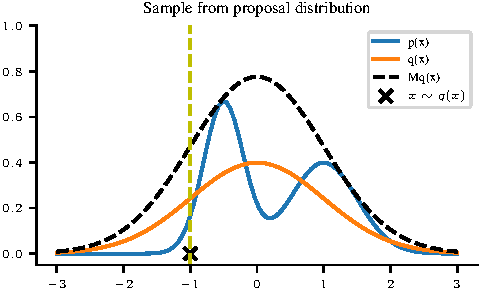
\includegraphics{notebooks/figures/sampling/rejection-sampling--1.0-True-True-True-True-False-False-False-False.pdf}
        \end{figure}
    \end{frame}

    \begin{frame}{Rejection Sampling}
        \begin{figure}
            \centering
            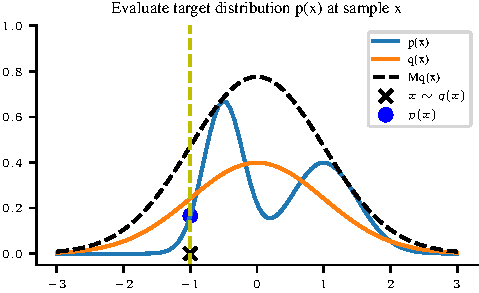
\includegraphics{notebooks/figures/sampling/rejection-sampling--1.0-True-True-True-True-True-False-False-False.pdf}
        \end{figure}
    \end{frame}

    \begin{frame}{Rejection Sampling}
        \begin{figure}
            \centering
            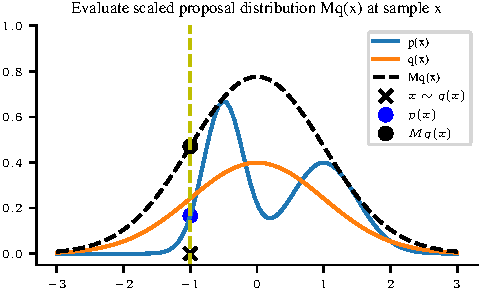
\includegraphics{notebooks/figures/sampling/rejection-sampling--1.0-True-True-True-True-True-True-False-False.pdf}
        \end{figure}
    \end{frame}

    \begin{frame}{Rejection Sampling}
        \begin{figure}
            \centering
            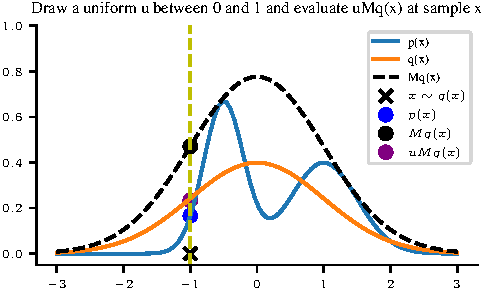
\includegraphics{notebooks/figures/sampling/rejection-sampling--1.0-True-True-True-True-True-True-True-False.pdf}
        \end{figure}
    \end{frame}

    \begin{frame}{Rejection Sampling}
        \begin{figure}
            \centering
            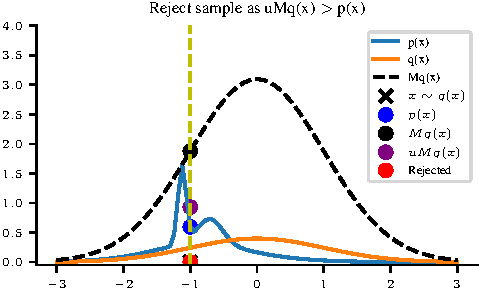
\includegraphics{notebooks/figures/sampling/rejection-sampling--1.0-True-True-True-True-True-True-True-True.pdf}
        \end{figure}
    \end{frame}

        
    
    \begin{frame}{Proof of Rejection Sampling}
        \begin{tcolorbox}[colback=metropolisblue!5,colframe=metropolisblue,title={Acceptance Probability $\alpha(x)$}]
            \begin{equation}
              \alpha(x) = \frac{p(x)}{M q(x)}
            \end{equation}
    \end{tcolorbox}
       
    \begin{tcolorbox}[colback=metropolisblue!5,colframe=metropolisblue,title={Bayes Rule for Acceptance}]
        \begin{equation}
            P(Sample|Accept) = \frac{P(Accept|Sample) P(Sample)}{P(Accept)}
        \end{equation}
\end{tcolorbox}

\begin{tcolorbox}[colback=metropolisblue!5,colframe=metropolisblue,title={P(Sample)}]
    We draw samples from $q(x)$, so $P(Sample) = q(x)$.
\end{tcolorbox}
\end{frame}

\begin{frame}{Proof of Rejection Sampling}
    


       
        

        Further, $P(Accept|Sample) = \alpha(x) = \dfrac{p(x)}{M q(x)}$.

        Finally, $P(Accept) = \int P(Accept|Sample) P(Sample) dSample = \int \alpha(x) q(x) dx = \dfrac{1}{M} \int p(x) dx = \dfrac{1}{M}$.
        \begin{tcolorbox}[colback=metropolisblue!5,colframe=metropolisblue,title={P(Accept)}]
            \begin{equation}
                P(Accept) = \frac{1}{M}
            \end{equation}
        \end{tcolorbox}
        

        Thus, $P(Sample|Accept) = \dfrac{p(x)}{M q(x)} \times \dfrac{q(x)}{1/M} = p(x)$.

        Thus, we have shown that the samples we accept are distributed according to $p(x)$.

        
    \end{frame}

    \begin{frame}{Rejection Sampling Completed Example}
        \begin{figure}
            \centering
            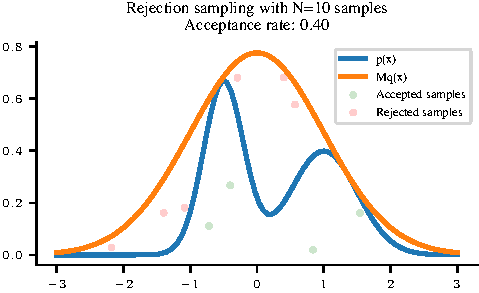
\includegraphics{notebooks/figures/sampling/rejection-sampling-N10-False.pdf}
        \end{figure}
        
    \end{frame}

    \begin{frame}{Rejection Sampling Completed Example}
        \begin{figure}
            \centering
            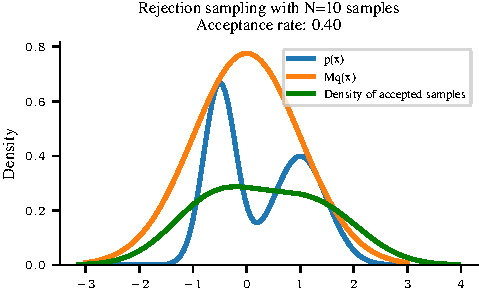
\includegraphics{notebooks/figures/sampling/rejection-sampling-N10-True.pdf}
        \end{figure}
        
    \end{frame}

    \begin{frame}{Rejection Sampling Completed Example}
        \begin{figure}
            \centering
            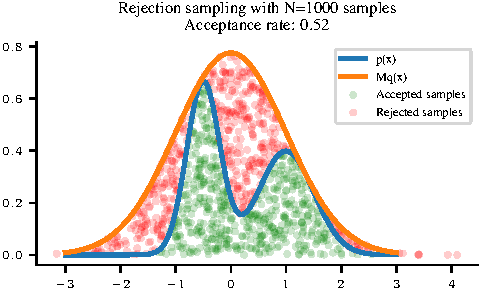
\includegraphics{notebooks/figures/sampling/rejection-sampling-N1000-False.pdf}
        \end{figure}
    \end{frame}

    \begin{frame}{Rejection Sampling Completed Example}
        \begin{figure}
            \centering
            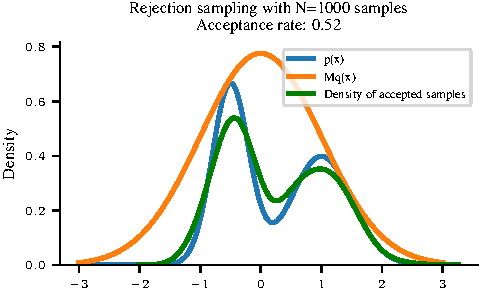
\includegraphics{notebooks/figures/sampling/rejection-sampling-N1000-True.pdf}
        \end{figure}
    \end{frame}

    \begin{frame}{Rejection Sampling Completed Example}
        \begin{figure}
            \centering
            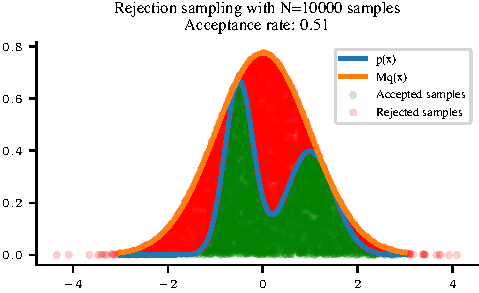
\includegraphics{notebooks/figures/sampling/rejection-sampling-N10000-False.pdf}
        \end{figure}
    \end{frame}

    \begin{frame}{Rejection Sampling Completed Example}
        \begin{figure}
            \centering
            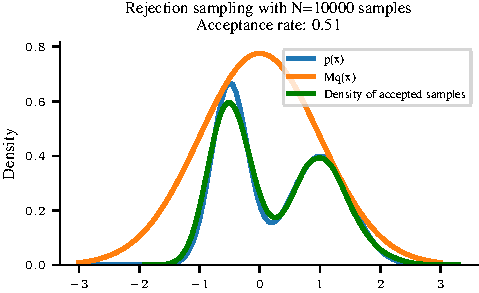
\includegraphics{notebooks/figures/sampling/rejection-sampling-N10000-True.pdf}
        \end{figure}
    \end{frame}
        

    \begin{frame}{Challenges with Rejection Sampling}
        \begin{itemize}
            \item Rejection sampling is inefficient when the target distribution is very different from the proposal distribution.
            \item In this case, we will reject a lot of samples.
            \item This is a problem when sampling from high-dimensional distributions.
            \item Acceptance probability $\alpha(x)$ is very low.
        \end{itemize}
        
    \end{frame}
    

\end{document}